\documentclass[11pt,a4paper]{article}

\usepackage[T1]{fontenc}
\usepackage[utf8]{inputenc}
\usepackage[margin=2.5cm]{geometry}
\usepackage{graphicx}
\usepackage{amsmath}
\usepackage{amssymb}
\usepackage{booktabs}
\usepackage{caption}
\usepackage{subcaption}
\usepackage{hyperref}
\usepackage{url}
\usepackage{float}

\title{MONET -- Supplementary Material \\ \large Benchmark Environments and Closed-Form Task Fitness Definitions}
\author{Julian Hatzky \and Thomas Bartz-Beielstein \and A.~E.\ Eiben \and Anil Yaman}
\date{}

\hypersetup{
  pdftitle={MONET Supplementary: Benchmark Environments and Fitness Definitions},
  pdfauthor={Hatzky, Bartz-Beielstein, Eiben, Yaman},
  colorlinks=true, linkcolor=blue, urlcolor=blue, citecolor=blue
}

\begin{document}
\maketitle

\noindent
This document accompanies the MONET paper \emph{``Multi-Task Optimization over
Networks of Tasks''} (Hatzky et al., 2026) and the code repository at
\url{https://github.com/ju2ez/MONET}. It collects the per-environment task /
solution parameterisations and the closed-form fitness expressions used in
the four benchmark domains.

\tableofcontents
\bigskip

\begin{figure}[H]
    \centering
    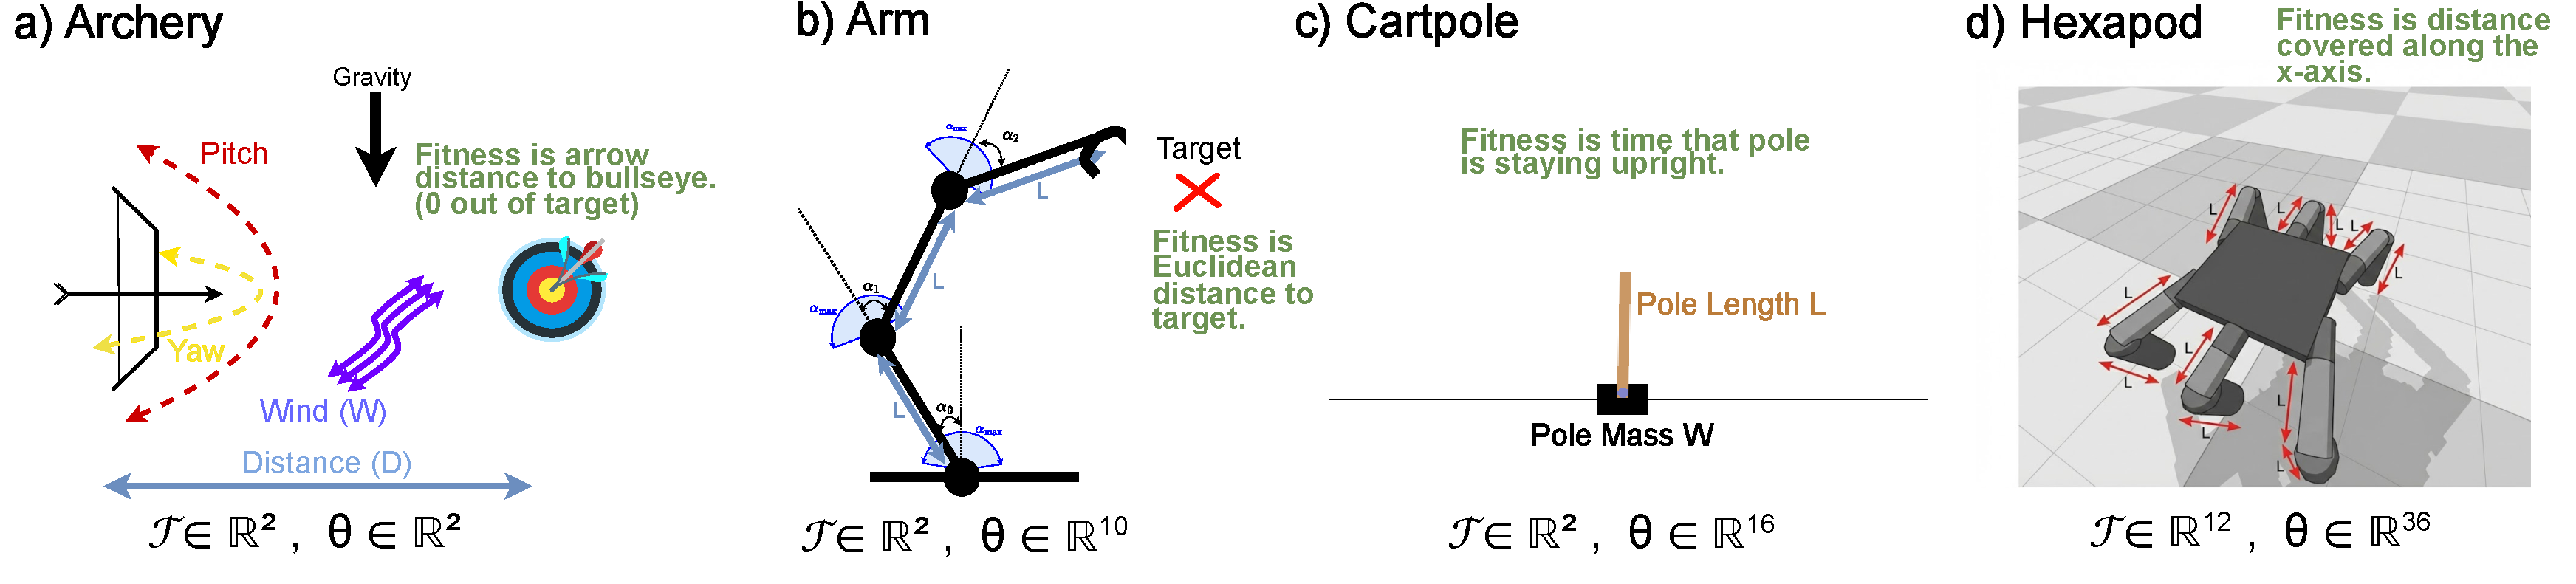
\includegraphics[width=0.95\textwidth]{figs/all_tasks_hor.pdf}
    \caption{Overview of benchmark environments used to evaluate MONET:
    (a) 10-DoF Arm, (b) Archery, (c) Cartpole with variable morphology,
    and (d) Six-legged locomotion (Hexapod).}
    \label{fig:benchmark-suite}
\end{figure}

All four benchmarks define fitness on $[0,1]$ (higher is better) and are
run for $10^{6}$ evaluations with a batch size of~$64$, replicated over
$20$ random seeds. Task parameters $\boldsymbol{\tau}\in\Theta$ define the
family of problems; solution vectors $\mathbf{x}\in\mathcal{X}$ are the
decision variables optimised per task.

\section{Benchmark Environments}\label{sec:envs}

\subsection{Kinematic Arm with Variable Morphology (10-DoF-Arm)}
A planar 10-DoF arm must place its end-effector at a fixed target
(Figure~\ref{fig:benchmark-suite}a); adapted from Mouret \&
Maguire~(2020).

\begin{description}
    \item[Tasks $\Theta$] maximum joint angle $\alpha_{\max}$ and link
    length~$L$.
    \item[Solutions $\mathcal{X}$] 10 joint angles, normalised by
    $\alpha_{\max}$.
    \item[Fitness] $\exp\!\bigl(-\lVert\mathbf{p}_{\text{ee}}-
        \mathbf{p}_{\text{tar}}\rVert^{2}\bigr)$.
    \item[Number of tasks] $5{,}000$.
\end{description}

\subsection{Archery with Adaptive Environment}
A projectile-aiming task in which the archer compensates for distance
and wind (Figure~\ref{fig:benchmark-suite}b); adapted from Anne \&
Mouret~(2024).

\begin{description}
    \item[Tasks $\Theta$] target distance $D\in[5,40]$\,m and horizontal
    wind $W\in[-10,10]\,\mathrm{m/s^2}$.
    \item[Solutions $\mathcal{X}$] arrow yaw and pitch, each in
    $[-\pi/12,\pi/12]$ at fixed launch speed $v_{0}=70\,\mathrm{m/s}$.
    \item[Fitness] normalised archery score derived from the analytic
    miss distance on the target plane.
    \item[Number of tasks] $5{,}000$.
\end{description}

\subsection{Cartpole with Variable Morphology}
Classic cart-pole balancing under varying physical parameters
(Figure~\ref{fig:benchmark-suite}c); Michie \& Chambers~(1968), Barto
et al.~(1983).

\begin{description}
    \item[Tasks $\Theta$] pole length $L\in[0.3,1.2]$\,m, pole mass
    $m_{p}\in[0.05,0.5]$\,kg, cart mass $m_{c}\in[0.2,2.0]$\,kg.
    \item[Solutions $\mathcal{X}$] control policy mapping state
    $(x_{c},\dot{x}_{c},\phi,\dot{\phi})$ to control force $F$.
    \item[Fitness] fraction of the episode during which the pole stays
    within $|\phi|<12^{\circ}$ and $|x_{c}|<2.4$\,m.
    \item[Number of tasks] $5{,}000$.
\end{description}

\subsection{Six-Legged Locomotion (Hexapod)}
A simulated hexapod must walk forward across varying body morphologies
(Figure~\ref{fig:benchmark-suite}d), simulated in PyBullet (Coumans \&
Bai, 2016--2021); adapted from Cully et al.~(2015) and Mouret \&
Maguire~(2020).

\begin{description}
    \item[Tasks $\Theta$] the 12 leg-segment lengths (2\,000 random
    morphologies).
    \item[Solutions $\mathcal{X}$] a 36-D gait vector encoding phase,
    amplitude, and offset of a smoothed square-wave trajectory for each
    of 12 controlled joints; the remaining 6 joints mirror their
    neighbours to keep the distal segment vertical.
    \item[Fitness] forward displacement $\Delta X$ over a 3\,s episode,
    normalised to $[0,1]$; episodes terminate early if body pitch/roll
    exceeds $\pi/8$ or lateral drift exceeds $0.5$\,m.
    \item[Number of tasks] $2{,}000$.
\end{description}

\section{Closed-Form Task Fitness Definitions}\label{sec:fitness}

This appendix gives the explicit fitness expressions for the four
benchmarks summarised in Section~\ref{sec:envs}.

\subsection{10-DoF Arm}
With end-effector position $\mathbf{p}_{\text{ee}}$ and target
$\mathbf{p}_{\text{tar}}$,
\[
f = \exp\!\left(-\lVert \mathbf{p}_{\text{ee}} - \mathbf{p}_{\text{tar}}
\rVert^{2}\right) \in [0,1].
\]

\subsection{Archery}
The initial velocity vector is
\[
\mathbf{v} = v_{0}
\begin{bmatrix}
-\sin(\text{yaw}) \\
\cos(\text{yaw})\cos(\text{pitch}) \\
\cos(\text{yaw})\sin(\text{pitch})
\end{bmatrix},
\qquad
t_{\text{hit}} = \frac{D}{v_{y}},
\]
and, with $g_{z}$ the gravitational acceleration along $z$ and $W_{x}$
the wind acceleration along $x$, the miss distance on the target plane
is
\[
r = \left\lVert \tfrac{1}{2}\!\left(-g_{z}\,\hat{\mathbf{e}}_{z}
      + W_{x}\,\hat{\mathbf{e}}_{x}\right)t_{\text{hit}}^{2}
      + \mathbf{v}\,t_{\text{hit}} \right\rVert_{2},
\qquad
f = \frac{\max\!\left(0,\,\operatorname{int}\!\left(10
    - \tfrac{r}{0.061}\right)\right)}{10}.
\]

\subsection{Cartpole}
With pole angle $\phi$, cart position $x_{c}$, control force $F$, and
gravity $g$,
\[
\ddot{\phi} = \frac{g \sin \phi + \cos \phi \left(-F - m_{p} L
   \dot{\phi}^{2} \sin \phi\right)/(m_{c} + m_{p})}
   {L \left(\tfrac{4}{3} - \tfrac{m_{p} \cos^{2}
   \phi}{m_{c} + m_{p}}\right)},
\]
\[
\ddot{x}_{c} = \frac{F + m_{p} L \left(\dot{\phi}^{2}
   \sin \phi - \ddot{\phi} \cos \phi\right)}{m_{c} + m_{p}}.
\]
Fitness is $f = t_{\text{balanced}}/t_{\text{max}}$, the fraction of the
episode the pole stays within $|\phi|<12^{\circ}$ and
$|x_{c}|<2.4\,\mathrm{m}$.

\subsection{Hexapod}
With gait parameters $\mathbf{x}\in\mathcal{X}$ and morphology
$\boldsymbol{\tau}\in\Theta$,
\[
f(\mathbf{x},\boldsymbol{\tau}) = \Delta X,
\]
the forward displacement of the centre of mass over a 3\,s episode
(normalised to~$[0,1]$), with early termination if body pitch or roll
exceeds $\pi/8$ or $|Y|>0.5\,\mathrm{m}$.

\section*{References (selected)}

\begin{itemize}\small
    \item Anne, T.\ and Mouret, J.-B.\ (2024).
    \emph{Parametric-Task MAP-Elites}. In \emph{Proc.\ GECCO 2024},
    pp.~68--77.
    \href{https://arxiv.org/abs/2402.01275}{arXiv:2402.01275} \textbullet{}
    \href{https://doi.org/10.1145/3638529.3654159}
    {doi:10.1145/3638529.3654159}.
    \item Barto, A.~G., Sutton, R.~S., and Anderson, C.~W.\ (1983).
    \emph{Neuronlike adaptive elements that can solve difficult learning
    control problems}. IEEE Trans.\ SMC, SMC-13(5):834--846.
    \href{https://doi.org/10.1109/TSMC.1983.6313077}
    {doi:10.1109/TSMC.1983.6313077}.
    \item Coumans, E.\ and Bai, Y.\ (2016--2021).
    \emph{PyBullet: a Python module for physics simulation for games,
    robotics and machine learning}.
    \href{https://pybullet.org}{pybullet.org} \textbullet{}
    \href{https://github.com/bulletphysics/bullet3}
    {github.com/bulletphysics/bullet3}.
    \item Cully, A., Clune, J., Tarapore, D., and Mouret, J.-B.\ (2015).
    \emph{Robots that can adapt like animals}. \emph{Nature} 521,
    503--507.
    \href{https://doi.org/10.1038/nature14422}
    {doi:10.1038/nature14422}.
    \item Michie, D.\ and Chambers, R.~A.\ (1968). \emph{BOXES: An
    experiment in adaptive control}. In \emph{Machine Intelligence 2}
    (E.\ Dale \& D.\ Michie, eds.), pp.~137--152. Oliver and Boyd,
    Edinburgh.
    \item Mouret, J.-B.\ and Maguire, G.\ (2020).
    \emph{Quality Diversity for Multi-Task Optimization}. In
    \emph{Proc.\ GECCO 2020}, pp.~121--129.
    \href{https://doi.org/10.1145/3377929.3390079}
    {doi:10.1145/3377929.3390079}.
\end{itemize}

\end{document}
